\documentclass[../main.tex]{subfiles}

\pagestyle{main}
\renewcommand{\chaptermark}[1]{\markboth{\chaptername\ \thechapter: #1}{}}
\setcounter{chapter}{5}

\begin{document}




\chapter{Inner Product Spaces}
\section{Inner Products and Norms}
\begin{itemize}
    \item \marginnote{9/30:}\textbf{Norm} (of $x\in\R^n$): The length of $x$. \emph{Denoted by} $\norm{x}$. \emph{Given by}
    \begin{equation*}
        \norm{x} = \sqrt{x_1^2+\cdots+x_n^2}
    \end{equation*}
    \item \textbf{Dot product} (of $x,y\in\R^n$): The quantity
    \begin{equation*}
        x\cdot y = x_1y_1+\cdots+x_ny_n
    \end{equation*}
    \item Properties of the dot product:
    \begin{itemize}
        \item $x\cdot x=\norm{x}^2$.
        \item $x\cdot x\geq 0$.
        \item $x\cdot x=0$ iff $x=0$.
        \item Let $y\in\R^n$. Then $T:\R^n\to\R$ defined by $Tx=x\cdot y$ is linear.
        \item $x\cdot y=y\cdot x$.
    \end{itemize}
    \item \textbf{Norm} (of $z\in\C^n$): The quantity
    \begin{equation*}
        \norm{z} = \sqrt{|z_1|^2+\cdots+|z_n|^2}
    \end{equation*}
    \begin{itemize}
        \item Note that $\norm{z}^2=z\cdot\bar{z}$.
    \end{itemize}
    \item \textbf{Inner product} (on $V$): A function that takes each ordered pair $(u,v)\in V$ to a number $\inp{u}{v}\in\F$ and has the following properties.
    \begin{description}
        \item[positivity] \hfill\\ $\inp{v}{v}\geq 0$ for all $v\in V$.
        \item[definiteness] \hfill\\ $\inp{v}{v}=0$ iff $v=0$.
        \item[additivity in first slot] \hfill\\ $\inp{u+v}{v}=\inp{u}{w}+\inp{v}{w}$ for all $u,v,w\in V$.
        \item[homogeneity in first slot] \hfill\\ $\inp{\lambda u}{v}=\lambda\inp{u}{v}$ for all $\lambda\in\F$ and all $u,v\in V$.
        \item[conjugate symmetry] \hfill\\ $\inp{u}{v}=\overline{\inp{v}{u}}$ for all $u,v\in V$.
    \end{description}
    \begin{itemize}
        \item Since every real number equals its complex conjugate, if $V$ is real, we can dispense with the conjugacy condition in the conjugate symmetry condition and just have $\inp{u}{v}=\inp{v}{u}$.
        \item \dq{Although most mathematicians define an inner product as above, many physicists use a definition that requires homogeneity in the second slot instead of the first}{166}
    \end{itemize}
    \item \textbf{Euclidean inner product} (on $\F^n$): The function defined by
    \begin{equation*}
        \inp{w}{z} = w_1\bar{z_1}+\cdots+w_n\bar{z_n}
    \end{equation*}
    \item \textbf{Inner product space}: A vector space $V$ along with an inner product on $V$.
    \begin{itemize}
        \item When $\F^n$ is referred to as an inner product space, assume that the inner product is the Euclidean inner product unless explicitly stated otherwise.
    \end{itemize}
    \item Basic properties of an inner product.
    \begin{theorem}\label{trm:inpProperties}\leavevmode
        \begin{enumerate}[label={\textup{(}\alph*\textup{)}},ref={\thetheorem\arabic*}]
            \item \label{trm:inpPropertiesa}For each fixed $u\in V$, the function that takes $v$ to $\inp{v}{u}$ is a linear map from $V$ to $\F$.
            \begin{proof}
                Let $u\in V$ be arbitrary, and let $T:V\to\F$ be defined by $Tv=\inp{v}{u}$. Let $v,w\in V$ be arbitrary, and let $\lambda\in\F$. Then
                \begin{align*}
                    T(v+w) &= \inp{v+w}{u}&
                        T(\lambda v) &= \inp{\lambda v}{u}\\
                    &= \inp{v}{u}+\inp{w}{u}&
                        &= \lambda\inp{v}{u}\\
                    &= Tv+Tw&
                        &= \lambda Tv
                \end{align*}
                as desired.
            \end{proof}
            \item \label{trm:inpPropertiesb}$\inp{0}{u}=0$ for every $u\in V$.
            \begin{proof}
                Let $u\in V$ be arbitrary. Since $T$ as defined above is linear, Theorem \ref{trm:linSendsZero} implies that $0=T(0)=\inp{0}{u}$, as desired.
            \end{proof}
            \item \label{trm:inpPropertiesc}$\inp{u}{0}=0$ for every $u\in V$.
            \begin{proof}
                Let $u\in V$ be arbitrary. By the conjugate symmetry property and the above, $\inp{u}{0}=\overline{\inp{0}{u}}=\bar{0}=0$, as desired.
            \end{proof}
            \item \label{trm:inpPropertiesd}$\inp{u}{v+w}=\inp{u}{v}+\inp{u}{w}$ for all $u,v,w\in V$.
            \begin{proof}
                Let $u,v,w\in V$ be arbitrary. Then
                \begin{align*}
                    \inp{u}{v+w} &= \overline{\inp{v+w}{u}}\\
                    &= \overline{\inp{v}{u}+\inp{w}{u}}\\
                    &= \overline{\inp{v}{u}}+\overline{\inp{w}{u}}\tag*{Theorem \ref{trm:propertiesComplex}}\\
                    &= \inp{u}{v}+\inp{v}{w}
                \end{align*}
                as desired.
            \end{proof}
            \item \label{trm:inpPropertiese}$\inp{u}{\lambda v}=\bar{\lambda}\inp{u}{v}$ for all $\lambda\in\F$ and $u,v\in V$.
            \begin{proof}
                Let $u,v\in V$, and let $\lambda\in\F$. Then
                \begin{align*}
                    \inp{u}{\lambda v} &= \overline{\inp{\lambda v}{u}}\\
                    &= \overline{\lambda\inp{v}{u}}\\
                    &= \bar{\lambda}\overline{\inp{v}{u}}\tag*{Theorem \ref{trm:propertiesComplex}}\\
                    &= \bar{\lambda}\inp{u}{v}
                \end{align*}
            \end{proof}
        \end{enumerate}
    \end{theorem}
    \item \textbf{Norm} (of $v\in V$): The quantity
    \begin{equation*}
        \norm{v} = \sqrt{\inp{v}{v}}
    \end{equation*}
    \item Basic properties of the norm.
    \begin{theorem}\label{trm:normProperties}
        Suppose $v\in V$. Then
        \begin{enumerate}[label={\textup{(}\alph*\textup{)}},ref={\thetheorem\alph*}]
            \item \label{trm:normPropertiesa}$\norm{v}=0$ iff $v=0$.
            \begin{proof}
                Suppose first that $\norm{v}=0$. Then $0=\sqrt{\inp{v}{v}}=\inp{v}{v}$. Thus, $v=0$. The proof is symmetric in the reverse direction.
            \end{proof}
            \item \label{trm:normPropertiesb}$\norm{\lambda v}=|\lambda|\norm{v}$ for all $\lambda\in\F$.
            \begin{proof}
                Let $\lambda\in\F$ be arbitrary. Then
                \begin{align*}
                    \norm{\lambda v}^2 &= \inp{\lambda v}{\lambda v}\\
                    &= \lambda\bar{\lambda}\inp{v}{v}\\
                    &= |\lambda|^2\norm{v}^2\tag*{Theorem \ref{trm:propertiesComplex}}
                \end{align*}
                Taking square roots of the above gives the desired equality.\footnote{Notice this technique: Working with norms squared is usually easier than working directly with norms.}
            \end{proof}
        \end{enumerate}
    \end{theorem}
    \item \textbf{Orthogonal} (vectors $u,v\in V$): Two vectors $u,v\in V$ such that $\inp{u}{v}=0$.\footnote{The word \emph{orthogonal} derives from the Greek word \emph{orthogonios}, which means right-angled.}
    \item If $u,v\in\R^2$ are nonzero, then $\inp{u}{v}=\norm{u}\norm{v}\cos\theta$.
    \begin{itemize}
        \item \dq{Thus, two vectors in $\R^2$ are orthogonal (with respect to the usual Euclidean inner product) if and only if the cosine of the angle between them is 0, which happens if and only if the vectors are perpendicular in the usual sense of plane geometry. Thus, you can think of the word \emph{orthogonal} as a fancy word meaning \emph{perpendicular}.}{169}
    \end{itemize}
    \item Orthogonality and zero.
    \begin{theorem}\leavevmode
        \begin{enumerate}[label={\textup{(}\alph*\textup{)}}]
            \item $0$ is orthogonal to every vector in $V$.
            \begin{proof}
                Let $u\in V$ be arbitrary. Then Theorem \ref{trm:inpPropertiesb} implies that $\inp{0}{u}=0$. Thus, $u$ and 0 are orthogonal, as desired.
            \end{proof}
            \item $0$ is the only vector in $V$ that is orthogonal to itself.
            \begin{proof}
                Let $v\in V$ be such that $v$ is orthogonal to itself. Then $\inp{v}{v}=0$. But by the property of definiteness, it follows that $v=0$, as desired.
            \end{proof}
        \end{enumerate}
    \end{theorem}
    \item The special case where $V=\R^2$ of the following is over $\num{2500}$ years old, although the following is not the original proof.
    \begin{theorem}[Pythagorean Theorem]\label{trm:pythagorean}
        Suppose $u,v\in V$ are orthogonal. Then
        \begin{equation*}
            \norm{u+v}^2 = \norm{u}^2+\norm{v}^2
        \end{equation*}
        \begin{proof}
            We have
            \begin{align*}
                \norm{u+v}^2 = \inp{u+v}{u+v}\\
                &= (\inp{u}{u}+\inp{u}{v})+(\inp{v}{u}+\inp{v}{v})\\
                &= \norm{u}^2+0+0+\norm{v}^2\\
                &= \norm{u}^2+\norm{v}^2
            \end{align*}
            as desired.
        \end{proof}
    \end{theorem}
    \begin{itemize}
        \item Note that we can prove the converse of the Pythagorean Theorem in \emph{real} inner product spaces as follows: If $\norm{u+v}^2=\norm{u}^2+\norm{v}^2$ for $u,v$ real, then
        \begin{align*}
            0 &= \inp{u}{v}+\inp{v}{u}\\
            &= \inp{u}{v}+\overline{\inp{u}{v}}\\
            &= 2\Re\inp{u}{v}\\
            &= \inp{u}{v}
        \end{align*}
        as desired.
    \end{itemize}
    \item Let $u,v\in V$ with $v\neq 0$. We are now equipped to consider how to write $u$ as the sum of $v$ plus a vector $w$ orthogonal to $v$, as in Figure \ref{fig:orthogonalDecomposition} below.
    \begin{theorem}\label{trm:orthogonalDecomposition}
        Suppose $u,v\in V$ with $v\neq 0$. Set $c=\frac{\inp{u}{v}}{\norm{v}^2}$ and $w=u-\frac{\inp{u}{v}}{\norm{v}^2}v$. Then $\inp{w}{v}=0$ and $u=cv+w$.
        \begin{figure}[h!]
            \centering
            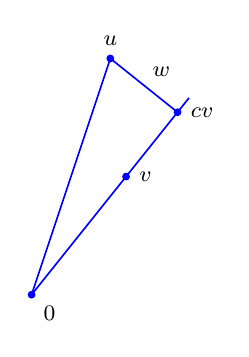
\begin{tikzpicture}[
                every path/.append style={blue,semithick},
                every node/.append style={black}
            ]
                \footnotesize
                \draw (0,0) node[circle,fill=blue,inner sep=1pt,label={below right:$0$}]{} -- (1,3) node[circle,fill=blue,inner sep=1pt,label={above:$u$}]{};
                \draw (0,0) -- node[pos=0.6,circle,fill=blue,inner sep=1pt,label={right:$v$}]{} (2,2.5);
                \draw ({76/41},{95/41}) node[circle,fill=blue,inner sep=1pt,label={right:$cv$}]{} -- node[above right]{$w$} (1,3);
            \end{tikzpicture}
            \caption{An orthogonal decomposition.}
            \label{fig:orthogonalDecomposition}
        \end{figure}
        \begin{proof}
            We want to write $u$ in the form $u=cv+w$ where $w$ is orthogonal to $v$. We know that
            \begin{equation*}
                u=cv+(u-cv)
            \end{equation*}
            so we need only choose $c$ such that $v$ is orthogonal to $u-cv$. In other words, we want
            \begin{align*}
                0 &= \inp{u-cv}{v}\\
                &= \inp{u}{v}+\inp{-cv}{v}\\
                &= \inp{u}{v}-c\inp{v}{v}\\
                &= \inp{u}{v}-c\norm{v}^2\\
                c &= \frac{\inp{u}{v}}{\norm{v}^2}
            \end{align*}
            But this gives the values we want for $c$ and $w$, as desired.
        \end{proof}
    \end{theorem}
    \item This allows for the proof of a very important result.
    \begin{theorem}[Cauchy-Schwarz Inequality]\label{trm:CauchySchwarz}
        Suppose $u,v\in V$. Then
        \begin{equation*}
            |\inp{u}{v}| \leq \norm{u}\norm{v}
        \end{equation*}
        This inequality is an equality if and only if one of $u,v$ is a scalar multiple of the other.
        \begin{proof}
            We divide into two cases ($v=0$ and $v\neq 0$). If $v=0$, then
            \begin{equation*}
                |\inp{u}{v}| = 0 \leq 0 = \norm{u}\sqrt{0} = \norm{u}\sqrt{\inp{u}{v}} = \norm{u}\norm{v}
            \end{equation*}
            and we also have that the equality holds since $v=0=0u$, $0\in\F$. Now let $v\neq 0$. Then by Theorem \ref{trm:orthogonalDecomposition},
            \begin{equation*}
                u = \frac{\inp{u}{v}}{\norm{v}^2}v+w
            \end{equation*}
            where $\inp{v}{w}=0$. It follows by the \hyperref[trm:pythagorean]{Pythagorean Theorem} that
            \begin{align*}
                \norm{u}^2 &= \norm{\frac{\inp{u}{v}}{\norm{v}^2}v}^2+\norm{w}^2\\
                &= \inp{\frac{\inp{u}{v}}{\norm{v}^2}v}{\frac{\inp{u}{v}}{\norm{v}^2}v}+\norm{w}^2\\
                &= \frac{\inp{u}{v}}{\norm{v}^2}\overline{\frac{\inp{u}{v}}{\norm{v}^2}}\inp{v}{v}+\norm{w}^2\\
                &= \frac{\inp{u}{v}\overline{\inp{u}{v}}}{\norm{v}^4}\norm{v}^2+\norm{w}^2\\
                &= \frac{|\inp{u}{v}|^2}{\norm{v}^2}+\norm{w}^2\\
                &\geq \frac{|\inp{u}{v}|^2}{\norm{v}^2}
            \end{align*}
            Multiplying both sides by $\norm{v}^2$ and taking square roots gives the desired inequality.\par
            Also note that the Cauchy-Schwarz inequality is an equality iff the last line is an equality, which happens iff $w=0$. But $w=0$ iff $u$ is a scalar multiple of $v$, as desired.
        \end{proof}
    \end{theorem}
    \item Note that the Cauchy-Schwarz is known as such because the French mathematician Augustin-Louis Cauchy proved the top inequality below in 1821, and the German mathematician Hermann Schwarz proved the bottom inequality below in 1886; both are special cases of the above.
    \begin{gather*}
        |x_1y_1+\cdots+x_ny_n|^2 \leq (x_1^2+\cdots+x_n^2)(y_1^2+\cdots+y_n^2)\\
        \left| \int_{-1}^1f(x)g(x)\dd{x} \right|^2 \leq \left( \int_{-1}^1(f(x))^2\dd{x} \right)\left( \int_{-1}^1(g(x))^2\dd{x} \right)
    \end{gather*}
    \begin{itemize}
        \item For the top one, we let $x_1,\dots,x_n,y_1,\dots,y_n\in\R$.
        \item For the bottom one, we let $f,g$ be continuous real-valued functions on $[-1,1]$.
    \end{itemize}
    \item We now prove another important inequality.
    \begin{theorem}[Triangle Inequality]
        Suppose $u,v\in V$. Then
        \begin{equation*}
            \norm{u+v} \leq \norm{u}+\norm{v}
        \end{equation*}
        This inequality is an equality if and only if one of $u,v$ is a nonnegative multiple of the other.
        \begin{proof}
            We have
            \begin{align*}
                \norm{u+v}^2 &= \inp{u+v}{u+v}\\
                &= \inp{u}{u}+\inp{v}{v}+\inp{u}{v}+\inp{v}{u}\\
                &= \inp{u}{u}+\inp{v}{v}+\inp{u}{v}+\overline{\inp{u}{v}}\\
                &= \norm{u}^2+\norm{v}^2+2\Re\inp{u}{v}\\
                &\leq \norm{u}^2+\norm{v}^2+2|\inp{u}{v}|\\
                &\leq \norm{u}^2+\norm{v}^2+2\norm{u}\norm{v}\tag*{\hyperref[trm:CauchySchwarz]{Cauchy-Schwarz Inequality}}\\
                &= (\norm{u}+\norm{v})^2
            \end{align*}
            Taking square roots of both sides gives the desired inequality.\par
            This inequality is an equality iff $\inp{u}{v}=\norm{u}\norm{v}$. Now suppose $u=cv$ where $c\in\F$ is positive. Then
            \begin{align*}
                \inp{u}{v} &= \inp{cv}{v}\\
                &= c\inp{v}{v}\\
                &= c\norm{v}^2\\
                &= c\sqrt{\inp{v}{v}}\norm{v}\\
                &= \sqrt{c^2\inp{v}{v}}\norm{v}\\
                &= \sqrt{\inp{cv}{cv}}\norm{v}\\
                &= \norm{u}\norm{v}
            \end{align*}
            The proof is the same in the reverse direction.
        \end{proof}
    \end{theorem}
    \item One last equality.
    \begin{theorem}[Parallelogram Equality]
        Suppose $u,v\in V$. Then
        \begin{equation*}
            \norm{u+v}^2+\norm{u-v}^2 = 2(\norm{u}^2+\norm{v}^2 )
        \end{equation*}
        \begin{figure}[h!]
            \centering
            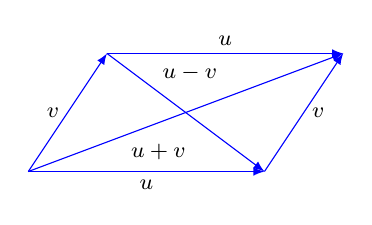
\begin{tikzpicture}[
                every path/.append style={blue,-latex},
                every node/.append style={black}
            ]
                \footnotesize
                \coordinate (a) at (0,0);
                \coordinate (b) at (3,0);
                \coordinate (c) at (4,1.5);
                \coordinate (d) at (1,1.5);

                \draw (a) -- node[below]{$u$} (b);
                \draw (b) -- node[right]{$v$} (c);
                \draw (d) -- node[above]{$u$} (c);
                \draw (a) -- node[left]{$v$}  (d);
                \draw (a) -- node[pos=0.3,below right]{$u+v$} (c);
                \draw (d) -- node[pos=0.3,above right]{$u-v$} (b);
            \end{tikzpicture}
            \caption{The parallelogram equality.}
            \label{fig:parallelogramEquality}
        \end{figure}
        \begin{proof}
            We have
            \begin{align*}
                \norm{u+v}^2+\norm{u-v}^2 &= \inp{u+v}{u+v}+\inp{u-v}{u-v}\\
                &= \norm{u}^2+\norm{v}^2+\inp{u}{v}+\inp{v}{u}+\norm{u}^2+\norm{v}^2-\inp{u}{v}-\inp{v}{u}\\
                &= 2(\norm{u}^2+\norm{v}^2)
            \end{align*}
            as desired.
        \end{proof}
    \end{theorem}
\end{itemize}



\section{Orthonormal Bases}
\begin{itemize}
    \item \marginnote{10/3:}\textbf{Orthonormal} (list of vectors): A list of vectors such that each vector in the list has norm 1 and is orthogonal to all the other vectors in the list.
    \begin{itemize}
        \item In other words, a list $e_1,\dots,e_m$ is orthonormal if
        \begin{equation*}
            \inp{e_j}{e_k} =
            \begin{cases}
                1 & j=k\\
                0 & j\neq k
            \end{cases}
        \end{equation*}
    \end{itemize}
    \item Orthonormal lists are particularly easy to work with.
    \begin{theorem}\label{trm:normOrthoLnlComb}
        If $e_1,\dots,e_m$ is an orthonormal list of vectors in $V$, then
        \begin{equation*}
            \norm{a_1e_1+\cdots+a_me_m}^2 = |a_1|^2+\cdots+|a_m|^2
        \end{equation*}
        for all $a_1,\dots,a_m\in\F$.
        \begin{proof}
            We have that
            \begin{align*}
                \norm{a_1e_1+\cdots+a_me_m}^2 &= \norm{a_1e_1}^2+\cdots+\norm{a_me_m}^2\tag*{\hyperref[trm:pythagorean]{Pythagorean Theorem}}\\
                &= |a_1|^2\norm{e_1}^2+\cdots+|a_m|^2\norm{e_m}^2\tag*{Theorem \ref{trm:normPropertiesb}}\\
                &= |a_1|^2+\cdots+|a_m|^2
            \end{align*}
            as desired.
        \end{proof}
    \end{theorem}
    \item The next result directly follows from the previous one.
    \begin{theorem}\label{trm:orthonormalLnlIndep}
        Every orthonormal list of vectors is linearly independent.
        \begin{proof}
            Let $e_1,\dots,e_m$ be an orthonormal list of vectors, and let $a_1,\dots,a_m\in\F$ be such that $a_1e_1+\cdots+a_me_m=0$. Then
            \begin{align*}
                0 &= \norm{0}\\
                &= \norm{a_1e_1+\cdots+a_me_m}\\
                &= |a_1|^2+\cdots+|a_m|^2\tag*{Theorem \ref{trm:normOrthoLnlComb}}
            \end{align*}
            But this implies that each $a_j=0$, as desired.
        \end{proof}
    \end{theorem}
    \item \textbf{Orthonormal basis} (of $V$): An orthonormal list of vectors in $V$ that is also a basis of $V$.
    \item We now prove an easy condition for identifying orthonormal bases.
    \begin{theorem}\label{trm:dimOrthonormal}
        Every orthonormal list of vectors in $V$ with length $\dim V$ is an orthonormal basis of $V$.
        \begin{proof}
            Let $e_1,\dots,e_m$ be an orthonormal list of vectors in $V$ with length $\dim V$. It follows by Theorem \ref{trm:orthonormalLnlIndep} that $e_1,\dots,e_m$ is linearly independent. Therefore, by Theorem \ref{trm:sameDimIndependent}, $e_1,\dots,e_m$ is a basis of $V$.
        \end{proof}
    \end{theorem}
    \item \marginnote{10/6:}For an arbitrary basis $e_1,\dots,e_n$ of $V$, it can be quite troublesome to compute that $a_1,\dots,a_n\in\F$ that make $a_1e_1+\cdots+a_ne_n=v$ for an arbitrary $v\in V$.
    \item However, it is quite simple for an orthonormal basis:
    \begin{theorem}\label{trm:linCombOrthonormal}
        Suppose $e_1,\dots,e_n$ is an orthonormal basis of $V$ and $v\in V$. Then
        \begin{equation*}
            v = \inp{v}{e_1}e_1+\cdots+\inp{v}{e_n}e_n
        \end{equation*}
        and
        \begin{equation*}
            \norm{v}^2 = |\inp{v}{e_1}|^2+\cdots+|\inp{v}{e_n}|^2
        \end{equation*}
        \begin{proof}
            Because $e_1,\dots,e_n$ is a basis of $V$, we have that
            \begin{equation*}
                v = a_1e_1+\cdots+a_ne_n
            \end{equation*}
            for some $a_1,\dots,a_n\in\F$. It follows by taking inner products with an arbitrary $e_j$ that
            \begin{align*}
                \inp{v}{e_j} &= \inp{a_1e_1+\cdots+a_ne_n}{e_j}\\
                &= a_1\inp{e_1}{e_j}+\cdots+a_n\inp{e_n}{e_j}\\
                &= a_1\cdot 0+\cdots+a_{j-1}\cdot 0+a_j\cdot 1+a_{j+1}\cdot 0+\cdots+a_n\cdot 0\\
                &= a_j
            \end{align*}
            for each $j=1,\dots,n$.\par
            The second equation follows from the first equation by Theorem \ref{trm:normOrthoLnlComb}.
        \end{proof}
    \end{theorem}
    \item The following algorithm\footnote{Danish mathematician J\o rgen Gram and German mathematician Erhard Schmidt popularized this algorithm.} gives a method for turning a linearly independent list into an orthonormal list with the same span as the original list.
    \begin{theorem}[Gram-Schmidt Procedure]\label{trm:GramSchmidt}
        Suppose $v_1,\dots,v_m$ is a linearly independent list of vectors in $V$. Let $e_1=v_1/\norm{v_1}$. For $j=2,\dots,m$, define $e_j$ inductively by
        \begin{equation*}
            e_j = \frac{v_j-\inp{v_j}{e_1}e_1-\cdots-\inp{v_j}{e_{j-1}}e_{j-1}}{\norm{v_j-\inp{v_j}{e_1}e_1-\cdots-\inp{v_j}{e_{j-1}}e_{j-1}}}
        \end{equation*}
        Then $e_1,\dots,e_m$ is an orthonormal list of vectors in $V$ such that
        \begin{equation*}
            \spn(v_1,\dots,v_j) = \spn(e_1,\dots,e_j)
        \end{equation*}
        for $j=1,\dots,m$.
        \begin{proof}
            We induct on $j$. For the base case $j=1$, we have that $e_1$ is trivially orthogonal to all other vectors in the list and that
            \begin{equation*}
                \norm{e_1} = \norm{\frac{v_1}{\norm{v_1}}}
                = \frac{1}{\norm{v_1}}\norm{v_1}
                = 1
            \end{equation*}
            proving that $e_1$ is an orthonormal list of vectors in $V$. Additionally, since $e_1$ is a scalar multiple of $v_1$, we naturally also have that
            \begin{equation*}
                \spn(v_1) = \spn(e_1)
            \end{equation*}\par\smallskip
            Now suppose inductively that we have proven that $e_1,\dots,e_j$ is an orthonormal list of vectors such that $\spn(v_1,\dots,v_j)=\spn(e_1,\dots,e_j)$. We now wish to prove the claim for $e_{j+1}$. To do so, it will suffice to show that $e_{j+1}$ is well defined, that $e_1,\dots,e_{j+1}$ is an orthonormal list of vectors, and that $\spn(v_1,\dots,v_{j+1})=\spn(e_1,\dots,e_{j+1})$. Let's begin.\par
            To confirm that the $e_{j+1}$ is well defined, we must confirm that the norm in the bottom is nonzero. But since $v_1,\dots,v_m$ is linearly independent by hypothesis, we have that $v_{j+1}\notin\spn(v_1,\dots,v_j)=\spn(e_1,\dots,e_j)$, meaning that we must have
            \begin{align*}
                v_{j+1} &\neq \inp{v_{j+1}}{e_1}e_1+\cdots+\inp{v_{j+1}}{e_j}e_j\\
                v_{j+1}-\inp{v_{j+1}}{e_1}e_1-\cdots-\inp{v_{j+1}}{e_j}e_j &\neq 0\\
                \norm{v_{j+1}-\inp{v_{j+1}}{e_1}e_1-\cdots-\inp{v_{j+1}}{e_j}e_j} &\neq 0\tag*{Theorem \ref{trm:normPropertiesa}}
            \end{align*}
            as desired.\par
            To confirm that $e_1,\dots,e_{j+1}$ is an orthonormal list of vectors, it will suffice to show that $e_{j+1}$ has norm 1 (the inductive hypothesis guarantees that $e_1,\dots,e_j$ have norm 1) and that each vector in $e_1,\dots,e_j$ is orthogonal to $e_{j+1}$ (again, we already know by the inductive hypothesis that $e_1,\dots,e_j$ is mutually orthogonal). We can address the first part with an argument symmetric to that used in the base case (indeed, it is easily seen that any vector divided by its norm has norm 1). As to the second part of the argument, we have for any $1\leq k<j+1$ that
            \begin{align*}
                \inp{e_{j+1}}{e_k} &= \inp{\frac{v_{j+1}-\inp{v_{j+1}}{e_1}e_1-\cdots-\inp{v_{j+1}}{e_j}e_j}{\norm{v_{j+1}-\inp{v_{j+1}}{e_1}e_1-\cdots-\inp{v_{j+1}}{e_j}e_j}}}{e_k}\\
                &= \frac{1}{\norm{v_{j+1}-\inp{v_{j+1}}{e_1}e_1-\cdots-\inp{v_{j+1}}{e_j}e_j}}(\inp{v_{j+1}}{e_k}-\inp{v_{j+1}}{e_1}\inp{e_1}{e_k}-\cdots-\inp{v_{j+1}}{e_j}\inp{e_j}{e_k})\\
                &= \frac{1}{\norm{v_{j+1}-\inp{v_{j+1}}{e_1}e_1-\cdots-\inp{v_{j+1}}{e_j}e_j}}(\inp{v_{j+1}}{e_k}-\inp{v_{j+1}}{e_k}\cdot 1)\\
                &= 0
            \end{align*}
            as desired.\par
            To confirm that $\spn(v_1,\dots,v_{j+1})=\spn(e_1,\dots,e_{j+1})$, Exercise \ref{exr:subspaceSameDim} tells us that it will suffice to show that $\spn(v_1,\dots,v_{j+1})\subset\spn(e_1,\dots,e_{j+1})$ and that $\dim\spn(v_1,\dots,v_{j+1})=\dim\spn(e_1,\dots,e_{j+1})$. Since $\spn(v_1,\dots,v_j)=\spn(e_1,\dots,e_j)$ by hypothesis, we have that $v_1,\dots,v_j\in\spn(e_1,\dots,e_j)\subset\spn(e_1,\dots,e_{j+1})$. Additionally, by the definition of $e_{j+1}$, we have that $v_{j+1}\in\spn(e_1,\dots,e_{j+1})$. Therefore, we have that
            \begin{equation*}
                \spn(v_1,\dots,v_{j+1}) \subset \spn(e_1,\dots,e_{j+1})
            \end{equation*}
            Additionally, since $v_1,\dots,v_{j+1}$ is linearly independent by hypothesis, and $e_1,\dots,e_{j+1}$ is linearly independent by Theorem \ref{trm:orthonormalLnlIndep}, we have that both subspaces have dimension $j+1$, as desired.
        \end{proof}
    \end{theorem}
    \item Existence of an orthonormal basis.
    \begin{theorem}
        Every finite-dimensional inner product space has an orthonormal basis.
        \begin{proof}
            Let $V$ be a finite-dimensional inner product space. Choose a basis of $V$. Applying the \hyperref[trm:GramSchmidt]{Gram-Schmidt Procedure} to this (by definition linearly independent) basis yields an orthonormal list of vectors in $V$ of length $\dim V$. Therefore, by Theorem \ref{trm:dimOrthonormal}, the orthonormal list is an orthonormal basis of $V$.
        \end{proof}
    \end{theorem}
    \item Extending an orthonormal list to an orthonormal basis.
    \begin{theorem}
        Suppose $V$ is finite-dimensional. Then every orthonormal list of vectors in $V$ can be extended to an orthonormal basis of $V$.
        \begin{proof}
            Suppose $e_1,\dots,e_m$ is an orthonormal list of vectors in $V$. Then by Theorem \ref{trm:orthonormalLnlIndep}, $e_1,\dots,e_m$ is linearly independent. Hence this list can be extended to a basis $e_1,\dots,e_m,v_1,\dots,v_n$ of $V$ by Theorem \ref{trm:lnlIndependentExtendBasis}. Applying the \hyperref[trm:GramSchmidt]{Gram-Schmidt Procedure} to this basis yields an orthonormal list $e_1,\dots,e_m,f_1,\dots,f_n$ of vectors in $V$. Note that the \hyperref[trm:GramSchmidt]{Gram-Schmidt Procedure} doesn't change the first $m$ vectors of the list: If $1\leq j\leq m$, then
            \begin{align*}
                e_j' &= \frac{e_j-\inp{e_j}{e_1}e_1-\cdots-\inp{e_j}{e_{j-1}}e_{j-1}}{\norm{e_j-\inp{e_j}{e_1}e_1-\cdots-\inp{e_j}{e_{j-1}}e_{j-1}}}\\
                &= \frac{e_j}{\norm{e_j}}\\
                &= e_j
            \end{align*}
            Lastly, by Theorem \ref{trm:dimOrthonormal}, we know that $e_1,\dots,e_m,f_1,\dots,f_n$ is a basis of $V$.
        \end{proof}
    \end{theorem}
    \item The next result build on Theorem \ref{trm:upperTriangularExists}.
    \begin{theorem}\label{trm:upperTriangularOrthonormal}
        Suppose $T\in\ope{V}$. If $T$ has an upper-triangular matrix with respect to some basis of $V$, then $T$ has an upper-triangular matrix with respect to some orthonormal basis of $V$.
        \begin{proof}
            Suppose $T$ has an upper-triangular matrix with respect to the basis $v_1,\dots,v_n$ of $V$. Then by Theorem \ref{trm:upperTriangularConditions}, $\spn(v_1,\dots,v_j)$ is invariant under $T$ for each $j=1,\dots,n$. Applying the \hyperref[trm:GramSchmidt]{Gram-Schmidt Procedure} to $v_1,\dots,v_n$, we obtain an orthonormal basis $e_1,\dots,e_n$ of $V$ with the property that
            \begin{equation*}
                \spn(e_1,\dots,e_j) = \spn(v_1,\dots,v_j)
            \end{equation*}
            for each $j=1,\dots,n$. Combining the last two results, we have that $\spn(e_1,\dots,e_j)$ is invariant under $T$ for each $j=1,\dots,n$. Therefore, by Theorem \ref{trm:upperTriangularConditions}, $T$ has an upper-triangular matrix with respect to the orthonormal basis $e_1,\dots,e_n$.
        \end{proof}
    \end{theorem}
    \item We now prove an important application of the above.
    \begin{theorem}[Schur's Theorem\footnote{German mathematician Issai Schur published the first proof of this result in 1909.}]
        Suppose $V$ is a finite-dimensional complex vector space and $T\in\ope{V}$. Then $T$ has an upper-triangular matrix with respect to some orthonormal basis of $V$.
        \begin{proof}
            By Theorem \ref{trm:upperTriangularExists}, $T$ has an upper-triangular matrix with respect to some basis of $V$. Therefore, by Theorem \ref{trm:upperTriangularOrthonormal}, $T$ has an upper-triangular matrix with respect to some orthonormal basis of $V$, as desired.
        \end{proof}
    \end{theorem}
    \item We now show that every linear functional is equivalent to some inner product.
    \begin{theorem}[Riesz Representation Theorem\footnote{This result is named for Hungarian mathematician Frigyes Riesz, who proved several results in the early twentieth century very similar to this one.}]\label{trm:RieszRepresentationTheorem}
        Suppose $V$ is finite-dimensional and $\varphi$ is a linear functional on $V$. Then there is a unique vector $u\in V$ such that
        \begin{equation*}
            \varphi(v) = \inp{v}{u}
        \end{equation*}
        for every $v\in V$.
        \begin{proof}
            We first find such a vector $u$. Let $e_1,\dots,e_n$ be an orthonormal basis of $V$. Then
            \begin{align*}
                \varphi(v) &= \varphi(\inp{v}{e_1}e_1+\cdots+\inp{v}{e_n}e_n)\tag*{Theorem \ref{trm:linCombOrthonormal}}\\
                &= \inp{v}{e_1}\varphi(e_1)+\cdots+\inp{v}{e_n}\varphi(e_n)\\
                &= \inp{v}{\overline{\varphi(e_1)}e_1+\cdots+\overline{\varphi(e_n)}e_n}\tag*{Theorem \ref{trm:inpPropertiese}}
            \end{align*}
            so we may take
            \begin{equation*}
                u = \overline{\varphi(e_1)}e_1+\cdots+\overline{\varphi(e_n)}e_n
            \end{equation*}\par
            Now suppose for the sake of contradiction that $u_1,u_2\in V$ are such that
            \begin{equation*}
                \varphi(v) = \inp{v}{u_1} = \inp{v}{u_2}
            \end{equation*}
            for every $v\in V$. Then
            \begin{equation*}
                0 = \inp{v}{u_1}-\inp{v}{u_2}
                = \inp{v}{u_1-u_2}
            \end{equation*}
            for every $v\in V$. In particular, if we let $v=u_1-u_2$, we have that $\inp{u_1-u_2}{u_1-u_2}=0$. Therefore, by the definiteness of the inner product, $u_1-u_2=0$, i.e., $u_1=u_2$, a contradiction.
        \end{proof}
    \end{theorem}
    \begin{itemize}
        \item Note that despite the fact that the expression for $u$ derived in the proof of the \hyperref[trm:RieszRepresentationTheorem]{Riesz Representation Theorem} seems to depend on both $\varphi$ and the chosen orthonormal basis, the statement of the theorem shows that the value of $u$ depends only on $\varphi$, and is in truth the same for any orthonormal basis.
    \end{itemize}
\end{itemize}



\section{Orthogonal Complements and Minimization Problems}
\begin{itemize}
    \item \textbf{Orthogonal complement} (of $U\subset V$): The set of all vectors in $V$ that are orthogonal to every vector in $U$. \emph{Denoted by} $\bm{U^\perp}$. \emph{Given by}
    \begin{equation*}
        U^\perp = \{v\in V:\inp{v}{u}=0\ \forall\ u\in U\}
    \end{equation*}
    \item Basic properties of the orthogonal complement.
    \begin{theorem}\label{trm:perpProperties}\leavevmode
        \begin{enumerate}[label={\textup{(}\alph*\textup{)}},ref={\thetheorem\alph*}]
            \item \label{trm:perpPropertiesa}If $U$ is a subset of $V$, then $U^\perp$ is a subspace of $V$.
            \begin{proof}
                Theorem \ref{trm:inpPropertiesb} tells us that $\inp{0}{u}=0$ for every $u\in U$; thus, $0\in U^\perp$, as desired.\par
                Let $v,w\in U^\perp$. Then
                \begin{equation*}
                    \inp{v+w}{u} = \inp{v}{u}+\inp{w}{u} = 0+0 = 0
                \end{equation*}
                for all $u\in U$. Thus, $v+w\in U^\perp$, as desired.\par
                Let $v\in U^\perp$ and $\lambda\in\F$. Then
                \begin{equation*}
                    \inp{\lambda v}{u} = \lambda\inp{v}{u} = \lambda\cdot 0 = 0
                \end{equation*}
                for all $u\in U$. Thus, $\lambda v\in U^\perp$, as desired.
            \end{proof}
            \item \label{trm:perpPropertiesb}$\{0\}^\perp=V$.
            \begin{proof}
                Let $v\in V$ be arbitrary. Then since $\inp{v}{0}=0$ by Theorem \ref{trm:inpPropertiesc}, we have that $v\in\{0\}^\perp$. Thus, $\{0\}^\perp=V$.
            \end{proof}
            \item \label{trm:perpPropertiesc}$V^\perp=\{0\}$.
            \begin{proof}
                Suppose $v\in V^\perp$. Then $\inp{v}{u}=0$ for all $u\in V$. In particular, $\inp{v}{v}=0$. But this implies that $v=0$ by the definiteness of the inner product. Therefore, $V^\perp=\{0\}$.
            \end{proof}
            \item \label{trm:perpPropertiesd}If $U$ is a subset of $V$, then $U\cap U^\perp\subset\{0\}$.
            \begin{proof}
                Let $v\in U\cap U^\perp$. Then $\inp{v}{v}=0$. Therefore, $U\cap U^\perp\subset\{0\}$.
            \end{proof}
            \item \label{trm:perpPropertiese}If $U$ and $W$ are subsets of $V$ and $U\subset W$, then $W^\perp\subset U^\perp$.
            \begin{proof}
                Let $v\in W^\perp$. Then $\inp{v}{u}=0$ for all $u\in W$. But since $U\subset W$, this implies that $\inp{v}{u}=0$ for all $u\in U$. Thus, $v\in U^\perp$. Therefore, $W^\perp\subset U^\perp$.
            \end{proof}
        \end{enumerate}
    \end{theorem}
    \item We can decompose $V$ into the direct sum of any subspace $U$ and another subspace.
    \begin{theorem}\label{trm:perpDirectSum}
        Suppose $U$ is a finite-dimensional subspace of $V$. Then
        \begin{equation*}
            V = U\oplus U^\perp
        \end{equation*}
        \begin{proof}
            First, we will show that any $v\in V$ can be written as the sum of an element of $U$ and an element of $U^\perp$. Then, we will show that this decomposition is unique. Let's begin.\par
            Let $v\in V$ be arbitrary, and let $e_1,\dots,e_m$ be an orthonormal basis of $U$. Then we may let
            \begin{equation*}
                v = \underbrace{\inp{v}{e_1}e_1+\cdots+\inp{v}{e_m}e_m}_u+\underbrace{v-\inp{v}{e_1}e_1-\cdots-\inp{v}{e_m}e_m}_w
            \end{equation*}
            Since $e_1,\dots,e_m$ is a basis of $U$, $u\in U$. Additionally, we have that
            \begin{align*}
                \inp{w}{e_j} &= \inp{v-\inp{v}{e_1}e_1-\cdots-\inp{v}{e_m}e_m}{e_j}\\
                &= \inp{v}{e_j}-\inp{v}{e_1}\inp{e_1}{e_j}-\cdots-\inp{v}{e_m}\inp{e_m}{e_j}\\
                &= \inp{v}{e_j}-\inp{v}{e_j}\cdot 1\\
                &= 0
            \end{align*}
            for all $e_j$. Thus, $w$ is orthogonal to every vector in $\spn(e_1,\dots,e_m)=U$. It follows that $w\in U^\perp$. Therefore, $v=u+w$ for $u\in U$ and $w\in U^\perp$, as desired.\par
            This combined with the fact that $U\cap U^\perp=\{0\}$ (by Theorem \ref{trm:perpPropertiesb}) implies that $V=U\oplus U^\perp$, as desired.
        \end{proof}
    \end{theorem}
    \item Dimension of the orthogonal complement.
    \begin{theorem}
        Suppose $V$ is finite-dimensional and $U$ is a subspace of $V$. Then
        \begin{equation*}
            \dim U^\perp = \dim V-\dim U
        \end{equation*}
        \begin{proof}
            By Theorem \ref{trm:perpDirectSum}, we have that $V=U\oplus U^\perp$. Therefore, by Theorem \ref{trm:dimDirectSum},
            \begin{align*}
                \dim V &= \dim U+\dim U^\perp\\
                \dim U^\perp &= \dim V-\dim U
            \end{align*}
            as desired.
        \end{proof}
    \end{theorem}
    \item We now have an important corollary to Theorem \ref{trm:perpDirectSum}.
    \begin{theorem}
        Suppose $U$ is a finite-dimensional subspace of $V$. Then
        \begin{equation*}
            U = (U^\perp)^\perp
        \end{equation*}
        \begin{proof}
            Suppose first that $u\in U$. Then $\inp{u}{v}=0$ for all $v\in U^\perp$ by the definition of $U^\perp$. But this also means that $u$ is orthogonal to every vector in $U^\perp$, i.e., that $u\in(U^\perp)^\perp$. Thus $U\subset(U^\perp)^\perp$.\par
            Now suppose that $v\in(U^\perp)^\perp$. By Theorem \ref{trm:perpDirectSum}, we have that $v=u+w$, where $u\in U$ and $w\in U^\perp$. It follows that $v-u=w\in U^\perp$ and, since $v\in(U^\perp)^\perp$ by hypothesis and $u\in(U^\perp)^\perp$ by the first part of the proof, that $v-u\in(U^\perp)^\perp$. Therefore, $v-u\in U^\perp\cap(U^\perp)^\perp\subset\{0\}$, so $v-u=0$ or $v=u\in U$, as desired.
        \end{proof}
    \end{theorem}
    \item \textbf{Orthogonal projection} (of $V$ onto $U$): The operator $P_U\in\ope{V}$ defined by $P_Uv=u$ iff $v=u+w$ where $u\in U$ and $w\in U^\perp$.
    \begin{itemize}
        \item Since Theorem \ref{trm:perpDirectSum} implies that each $v\in V$ can be written uniquely in the form $u+w$ where $u\in U$ and $w\in U^\perp$ for any subspace $U$ of $V$, $P_Uv$ is well defined in general.
    \end{itemize}
    \item Properties of the orthogonal projection.
    \begin{theorem}\label{trm:projProperties}
        Suppose $U$ is a finite-dimensional subspace of $V$ and $v\in V$. Then
        \begin{enumerate}[label={\textup{(}\alph*\textup{)}},ref={\thetheorem\alph*}]
            \item \label{trm:projPropertiesa}$P_U\in\ope{V}$.
            \begin{proof}
                To prove that $P_U$ is a linear map on $V$, suppose $v_1,v_2\in V$ and $a_1,a_2\in\F$. Let
                \begin{align*}
                    v_1 &= u_1+w_1&
                    v_2 &= u_2+w_2
                \end{align*}
                where $u_1,u_2\in U$ and $w_1,w_2\in U^\perp$. Then
                \begin{align*}
                    P_U(a_1v_1+a_2v_2) &= P_U(a_1u_1+a_2u_2+a_1w_1+a_2w_2)\\
                    &= a_1u_1+a_2u_2\\
                    &= a_1P_uv_1+a_2P_2v_2
                \end{align*}
                as desired.
            \end{proof}
            \item \label{trm:projPropertiesb}$P_Uu=u$ for every $u\in U$.
            \begin{proof}
                Let $u\in U$ be arbitrary. Then $u=u+0$ where $u\in U$ and $0\in U^\perp$. Thus, $P_Uu=u$.
            \end{proof}
            \item \label{trm:projPropertiesc}$P_Uw=0$ for every $w\in U^\perp$.
            \begin{proof}
                Let $w\in U^\perp$. Then $w=0+w$ where $0\in U$ and $w\in U^\perp$. Thus, $P_Uw=0$.
            \end{proof}
            \item \label{trm:projPropertiesd}$\range P_U=U$.
            \begin{proof}
                By the definition of $P_U$, $\range P_U\subset U$. Additionally, by Theorem \ref{trm:projPropertiesb}, $U\subset\range P_U$. Thus, $\range P_U=U$, as desired.
            \end{proof}
            \item \label{trm:projPropertiese}$\null P_U=U^\perp$.
            \begin{proof}
                Theorem \ref{trm:projPropertiesc} implies that $U^\perp\subset\null P_U$. In the other direction, we have that if $v\in\null P_U$, then $P_Uv=0$. Thus, we must have $v=0+v$, where $0\in U$ and $v\in U^\perp$. Consequently, $\null P_U\subset U^\perp$. Therefore, $\null P_U=U^\perp$, as desired.
            \end{proof}
            \item \label{trm:projPropertiesf}$v-P_Uv\in U^\perp$.
            \begin{proof}
                If $v=u+w$ with $u\in U$ and $w\in U^\perp$, then $v-P_Uv=v-u=w\in U^\perp$, as desired.
            \end{proof}
            \item \label{trm:projPropertiesg}$P_U^2=P_U$.
            \begin{proof}
                If $v-u+w$ with $u\in U$ and $w\in U^\perp$, then $(P_U^2)v=P_U(P_Uv)=P_Uu=u=P_Uv$, as desired.
            \end{proof}
            \item \label{trm:projPropertiesh}$\norm{P_Uv}\leq\norm{v}$.
            \begin{proof}
                If $v=u+w$ with $u\in U$ and $w\in U^\perp$, then
                \begin{align*}
                    \norm{P_Uv} &= \norm{u}^2\\
                    &\leq \norm{u}^2+\norm{w}^2\\
                    &= \norm{v}^2\tag*{\hyperref[trm:pythagorean]{Pythagorean Theorem}}
                \end{align*}
                Taking square roots gives the desired inequality.
            \end{proof}
            \item \label{trm:projPropertiesi}For every orthonormal basis $e_1,\dots,e_m$ of $U$,
            \begin{equation*}
                P_Uv = \inp{v}{e_1}e_1+\cdots+\inp{v}{e_m}e_m
            \end{equation*}
            \begin{proof}
                If $v=u+w$ with $u\in U$ and $w\in U^\perp$, then
                \begin{align*}
                    P_Uv &= u\\
                    &= \inp{v}{e_1}e_1+\cdots+\inp{v}{e_m}e_m\tag*{Theorem \ref{trm:linCombOrthonormal}}
                \end{align*}
                as desired.
            \end{proof}
        \end{enumerate}
    \end{theorem}
    \item Minimizing the distance to a subspace.
    \begin{theorem}
        Suppose $U$ is a finite-dimensional subspace of $V$, $v\in V$, and $u\in U$. Then
        \begin{equation*}
            \norm{v-P_Uv} \leq \norm{v-u}
        \end{equation*}
        Furthermore, the inequality above is an equality if and only if $u=P_Uv$.
        \begin{proof}
            We have
            \begin{align*}
                \norm{v-P_Uv}^2 &\leq \norm{v-P_Uv}^2+\norm{P_Uv-u}^2\\
                &= \norm{(v-P_Uv)+(P_Uv-u)}^2\tag*{\hyperref[trm:pythagorean]{Pythagorean Theorem}}\\
                &= \norm{v-u}^2
            \end{align*}
            Taking square roots of the above give the desired inequality.\par
            The inequality is an equality if and only if $\norm{P_Uv-u}^2=0$. But this happens if and only if $u=P_Uv$, as desired.
        \end{proof}
    \end{theorem}
    \begin{itemize}
        \item The above theorem is often combined with Theorem \ref{trm:projPropertiesi} to compute explicit solutions to minimization problems.
    \end{itemize}
\end{itemize}




\end{document}